\documentclass[man]{apa6}

\usepackage{amssymb,amsmath}
\usepackage{ifxetex,ifluatex}
\usepackage{fixltx2e} % provides \textsubscript
\ifnum 0\ifxetex 1\fi\ifluatex 1\fi=0 % if pdftex
  \usepackage[T1]{fontenc}
  \usepackage[utf8]{inputenc}
\else % if luatex or xelatex
  \ifxetex
    \usepackage{mathspec}
    \usepackage{xltxtra,xunicode}
  \else
    \usepackage{fontspec}
  \fi
  \defaultfontfeatures{Mapping=tex-text,Scale=MatchLowercase}
  \newcommand{\euro}{€}
\fi
% use upquote if available, for straight quotes in verbatim environments
\IfFileExists{upquote.sty}{\usepackage{upquote}}{}
% use microtype if available
\IfFileExists{microtype.sty}{\usepackage{microtype}}{}

% Table formatting
\usepackage{longtable, booktabs}
\usepackage{lscape}
% \usepackage[counterclockwise]{rotating}   % Landscape page setup for large tables
\usepackage{multirow}		% Table styling
\usepackage{tabularx}		% Control Column width
\usepackage[flushleft]{threeparttable}	% Allows for three part tables with a specified notes section
\usepackage{threeparttablex}            % Lets threeparttable work with longtable

% Create new environments so endfloat can handle them
% \newenvironment{ltable}
%   {\begin{landscape}\begin{center}\begin{threeparttable}}
%   {\end{threeparttable}\end{center}\end{landscape}}

\newenvironment{lltable}
  {\begin{landscape}\begin{center}\begin{ThreePartTable}}
  {\end{ThreePartTable}\end{center}\end{landscape}}

  \usepackage{ifthen} % Only add declarations when endfloat package is loaded
  \ifthenelse{\equal{\string man}{\string man}}{%
   \DeclareDelayedFloatFlavor{ThreePartTable}{table} % Make endfloat play with longtable
   % \DeclareDelayedFloatFlavor{ltable}{table} % Make endfloat play with lscape
   \DeclareDelayedFloatFlavor{lltable}{table} % Make endfloat play with lscape & longtable
  }{}%



% The following enables adjusting longtable caption width to table width
% Solution found at http://golatex.de/longtable-mit-caption-so-breit-wie-die-tabelle-t15767.html
\makeatletter
\newcommand\LastLTentrywidth{1em}
\newlength\longtablewidth
\setlength{\longtablewidth}{1in}
\newcommand\getlongtablewidth{%
 \begingroup
  \ifcsname LT@\roman{LT@tables}\endcsname
  \global\longtablewidth=0pt
  \renewcommand\LT@entry[2]{\global\advance\longtablewidth by ##2\relax\gdef\LastLTentrywidth{##2}}%
  \@nameuse{LT@\roman{LT@tables}}%
  \fi
\endgroup}


  \usepackage{graphicx}
  \makeatletter
  \def\maxwidth{\ifdim\Gin@nat@width>\linewidth\linewidth\else\Gin@nat@width\fi}
  \def\maxheight{\ifdim\Gin@nat@height>\textheight\textheight\else\Gin@nat@height\fi}
  \makeatother
  % Scale images if necessary, so that they will not overflow the page
  % margins by default, and it is still possible to overwrite the defaults
  % using explicit options in \includegraphics[width, height, ...]{}
  \setkeys{Gin}{width=\maxwidth,height=\maxheight,keepaspectratio}
\ifxetex
  \usepackage[setpagesize=false, % page size defined by xetex
              unicode=false, % unicode breaks when used with xetex
              xetex]{hyperref}
\else
  \usepackage[unicode=true]{hyperref}
\fi
\hypersetup{breaklinks=true,
            pdfauthor={},
            pdftitle={Developing a digital marketplace for family planning: Results of a pilot randomized encouragement trial},
            colorlinks=true,
            citecolor=blue,
            urlcolor=blue,
            linkcolor=black,
            pdfborder={0 0 0}}
\urlstyle{same}  % don't use monospace font for urls

\setlength{\parindent}{0pt}
%\setlength{\parskip}{0pt plus 0pt minus 0pt}

\setlength{\emergencystretch}{3em}  % prevent overfull lines


% Manuscript styling
\captionsetup{font=singlespacing,justification=justified}
\usepackage{csquotes}
\usepackage{upgreek}

 % Line numbering
  \usepackage{lineno}
  \linenumbers


\usepackage{tikz} % Variable definition to generate author note

% fix for \tightlist problem in pandoc 1.14
\providecommand{\tightlist}{%
  \setlength{\itemsep}{0pt}\setlength{\parskip}{0pt}}

% Essential manuscript parts
  \title{Developing a digital marketplace for family planning: Results of a pilot
randomized encouragement trial}

  \shorttitle{Family Planning}


  \author{Eric P Green, Ph.D.\textsuperscript{1}, Arun Augustine\textsuperscript{1}, \& Violet Naanyu, Ph.D.\textsuperscript{2}}

  % \def\affdep{{"", "", ""}}%
  % \def\affcity{{"", "", ""}}%

  \affiliation{
    \vspace{0.5cm}
          \textsuperscript{1} Duke Global Health Institute, Duke University\\
          \textsuperscript{2} Department of Behavioral Sciences, School of Medicine, College of Health
Sciences, Moi University  }

  \authornote{
    Correspondence concerning this article should be addressed to Eric P
    Green, Ph.D., . E-mail:
    \href{mailto:eric.green@duke.edu}{\nolinkurl{eric.green@duke.edu}}
  }


  \abstract{\textbf{Background:} Family planning is an effective tool for preventing
death among women who do not want to become pregnant and has also been
shown to improve newborn health outcomes, advance women's empowerment,
and bring socioeconomic benefits through reductions in fertility and
population growth. Yet among the populations that would benefit the most
from family planning, uptake remains too low. The emergence of digital
health tools have created new opportunities to strengthen health systems
and promote behavior change. In this study, women with an unmet need for
family planning in Western Kenya were randomized to receive an
encouragement to try an investigational digital health intervention.
\newline \textbf{Objective:} The objectives of the pilot study were to
explore the feasibility of a full-scale trial---in particular the
recruitment, encouragement, and follow-up data collection
procedures---and to examine the preliminary effect of the intervention
on the take-up of contraception. \newline \textbf{Methods:} This pilot
study tested the procedures for a randomized encouragement trial. We
recruited 112 women with an unmet need for family planning from local
markets in Western Kenya, conducted an eligibility screening, and
randomized half of the women to receive an encouragement to try the
investigational intervention. Four months after encouraging the
treatment group, we attempted to conduct a follow-up survey with all
enrolled participants. \newline \textbf{Results:} The encouragement sent
via text message to the treatment group led to differential rates of
intervention uptake between the treatment and control groups, but
take-up among the treatment group was lower than anticipated (33.9\% vs
1.8\% in the control group). Study attrition was also substantial. We
obtained follow-up data from 44.6\% of enrolled participants. Among
those in the treatment group who tried the intervention, however,
instrumental variables estimate of the Local Average Treatment Effect
was an increase in the probability of contraceptive take-up of 41.0
percentage points. \newline \textbf{Conclusions:} This randomized
encouragement design and study protocol is feasible but requires
modifications to the encouragement and follow-up data collection
procedures. The investigational intervention appears to have a positive
impact on contraceptive take-up among women with an unmet need despite a
number of contextual challenges. \newline \textbf{Pilot Trial
Registration:} ClinicalTrials.gov NCT03224390.}
  \keywords{family planning, unmet need, contraception, digital health, Kenya \\

    
  }




  \usepackage{pdfpages}
  \usepackage{setspace}
  \AtBeginEnvironment{tabular}{\singlespacing}
  \makeatletter
  
  \let\expandableinput\@@input
  
  \makeatother
  \interfootnotelinepenalty=10000

\usepackage{amsthm}
\newtheorem{theorem}{Theorem}[section]
\newtheorem{lemma}{Lemma}[section]
\theoremstyle{definition}
\newtheorem{definition}{Definition}[section]
\newtheorem{corollary}{Corollary}[section]
\newtheorem{proposition}{Proposition}[section]
\theoremstyle{definition}
\newtheorem{example}{Example}[section]
\theoremstyle{definition}
\newtheorem{exercise}{Exercise}[section]
\theoremstyle{remark}
\newtheorem*{remark}{Remark}
\newtheorem*{solution}{Solution}
\begin{document}

\maketitle

\setcounter{secnumdepth}{0}



\hypertarget{introduction}{%
\section{Introduction}\label{introduction}}

Pregnancy exposes women to the risk of maternal death, and family
planning is an effective tool for preventing death among women who do
not want to become pregnant {[}1{]}. First, by preventing unintended
pregnancies, contraception use reduces deaths caused by unsafe
abortions. Second, contraception use leads to fewer high-risk
pregnancies among adolescents and women over the age of 35. For the
12-month period ending July 2017, contraceptive use across 69 focal
countries included in the global initiative FP2020 is estimated to have
prevented 84 million unintended pregnancies, averted 26 million unsafe
abortions, and saved 125,000 women from maternal deaths {[}2{]}.
Voluntary family planning has also been shown to improve newborn health
outcomes, advance women's empowerment, and bring socioeconomic benefits
through reductions in fertility and population growth {[}1{]}.

Yet among the populations that would benefit the most from family
planning, uptake remains too low. In the five years that have passed
since the FP2020 initiative launched at the London Summit on Family
Planning in 2012, an additional 38.8 million women and girls across the
69 focal countries began using a modern method of contraception {[}2{]}.
This progress is above historic trends, but substantially off the pace
required to meet the goal of adding 120 million new users by 2020.
Across these focal countries, 1 out of every 5 married women of
reproductive age would like to prevent or delay childbirth but is not
using a modern method of contraception.

This indicator is referred to as unmet need for modern contraception,
and it represents a measure of access to family planning. In Kenya, for
instance, 17.2\% of currently married or in-union women of reproductive
age {[}3{]} and 26.4\% of sexually active unmarried women {[}4{]} have
an unmet need for family planning. This translates into approximately
1.3 million women in the country who are not using contraception but say
they would like to avoid pregnancy.\footnote{In the 2014 Kenya DHS,
  59.7\% of women ages 15 to 49 were classified as married or in-union
  and 1.9\% unmarried but sexually active. The current population of
  women ages 15 to 49 is approximately 11.8 million.} According to the
same nationally representative study, millions of others are either
unaware of the potential benefits of contraception, misinformed about
the full range of modern methods available, or unsatisfied with previous
experiences using contraception. Taken together, this presents a
promising opportunity to significantly reduce the current unmet need for
family planning and to expand the market.

Traditional approaches to promoting the take-up of family planning focus
on demand generation activities, and supply-side activities, or a
mixture of both. Demand generation can include mass media advertising,
interpersonal communication, and development approaches such as
conditional cash transfer programs. Supply-side interventions often
include efforts to improve service access, quality, and cost. A
systematic review of 63 published evaluations of family planning
interventions concluded that development approaches and supply-side
interventions had the most consistent effect on contraceptive use
{[}5{]}, but the overall quality of the evidence was low.

The emergence of digital health tools such as short message service
(SMS), interactive voice response, and smartphone applications have
created new opportunities to strengthen health systems and promote
behavior change {[}6,7{]}, but the evidence base remains weak. As is the
case in non-digital interventions {[}5{]}, studies of digital health
tools have found that it is easier to increase knowledge than it is to
achieve behavior change {[}8{]}.

This pilot study represents another effort to promote behavior change
through the use of an SMS intervention. Women with an unmet need for
family planning in Western Kenya were randomized to receive an
encouragement to try an investigational digital health intervention. The
objectives of the pilot study were to explore the feasibility of a
full-scale trial---in particular the recruitment, encouragement, and
follow-up data collection procedures---and to examine the preliminary
effect of the intervention on the take-up of contraception.

\hypertarget{methods}{%
\section{Methods}\label{methods}}

This was an external pilot study {[}9,10{]} conducted to inform the
design and implementation of a separate full-scale trial. The study
design was a randomized encouragement trial.

\hypertarget{setting-and-participants}{%
\subsection{Setting and Participants}\label{setting-and-participants}}

The target population for this study was Kenyan women who had an unmet
need for family planning; that is, women who were not using family
planning but wished to delay or prevent pregnancy. The accessible
population was limited to women with an unmet need living in Bungoma
county, Kenya.

\hypertarget{recruitment-and-eligibility-screening}{%
\subsubsection{Recruitment and eligibility
screening}\label{recruitment-and-eligibility-screening}}

Over a period of 4 weeks in 2017, from July 12 until August 6, we
conducted recruitment exercises five days per week at 1 of 6 open-air
markets throughout the county.\footnote{We identified 21 primary (10)
  and secondary (11) market venues in Bungoma county and selected 5
  primary and 1 secondary markets that maximized geographical coverage
  and market volume. We visited each market on its \enquote{market day},
  the day of the week when foot traffic peaks. Market days for the
  selected markets were Sunday, Monday, Wednesday, Thursday, and Friday.
  Our team visited two markets on Fridays.} Our market stall advertised
an opportunity to participate in the \enquote{Bungoma County Women's
Health Study}. A team of four female study team members, all Kenyan,
staffed the study table and screened women for eligibility.

To be eligible to enroll in the study, women had to meet several
criteria: (a) be between the ages of 18 and 35 (inclusive); (b) have an
unmet need for family planning; (c) live in Bungoma county; (d)
demonstrate phone ownership; (e) opt-in to receiving calls and/or SMS
messages related to the study; (f) demonstrate basic ability to operate
study tablet; and (g) consent to participate in the study. Women who
were pregnant or less than four months postpartum were excluded.

To begin the screening with an interested woman, a member of the study
team asked the woman her age and her county of residence. To continue to
the second stage of screening, the woman had to show the enumerator that
she received a test SMS message from the study shortcode. In the second
phase of screening, the enumerator asked the woman if she was pregnant
or currently using any method of family planning to prevent or delay
pregnancy.

If the woman was eligible to move to the third stage of screening, the
enumerator demonstrated how to use the tablet computer to complete the
survey via ACASI (audio computer assisted self-interview). The screening
survey text and audio was available in English and Swahili. The woman
had to demonstrate proficiency in an example exercise to continue to the
full screening. Enumerators were on hand to assist participants who
needed help using the tablet.

\hypertarget{unmet-need}{%
\subsubsection{Unmet need}\label{unmet-need}}

In the third and final phase of screening, the woman completed the
baseline survey to enable us to classify her unmet need status and to
collect relevant background information. The baseline survey instrument
included several modules from the 2014 Kenya Demographic and Health
Survey (Phase 7, short form), including household characteristics,
respondent's background, reproduction, contraception, and marriage and
sexual activity {[}3{]}.

In defining unmet need for this study, we followed guidelines published
by the Demographic and Health Survey Program (DHS, revised 2012)
{[}11{]} and other relevant scholarly reviews {[}12{]}. A woman was
classified as having an unmet need if she reported no current use of
contraception, was not identified by the survey as infecund, and said
she did not want to be pregnant for at least two years. A woman could
also be classified as having an unmet need if she was postpartum
amenorrheic and reported that she did not want her last birth at all or
wanted to become pregnant later than she did. We further classified
women as having an unmet need for limiting (does not want to become
pregnant at all) or spacing (wants to delay pregnancy for at least two
years). We also extended this classification of unmet need to woman who
were not married or in a union if they reported being sexually active in
the past month, thus making them at risk for pregnancy. See our
Supplementary Materials for survey questions and a detailed algorithm
for determining unmet need.

\hypertarget{enrollment}{%
\subsubsection{Enrollment}\label{enrollment}}

If the woman was eligible to participate in the study based on her
responses to the screening, the tablet prompted the enumerator to review
the informed consent form with her. If she consented to participate, the
enumerator recorded her name and contact details in the study register.
Every woman who completed the screening received an honorarium of Ksh
200 (approximately USD \$2) to appreciate her time and effort,
regardless of whether she was eligible to participate in the study or
consented to participate. Ineligible women were not informed about the
specific reason that they were ineligible to prevent others from
determining what answers would trigger eligibility. See the participant
flow diagram presented in Figure \ref{fig:flow} for details.

\begin{figure}
\centering
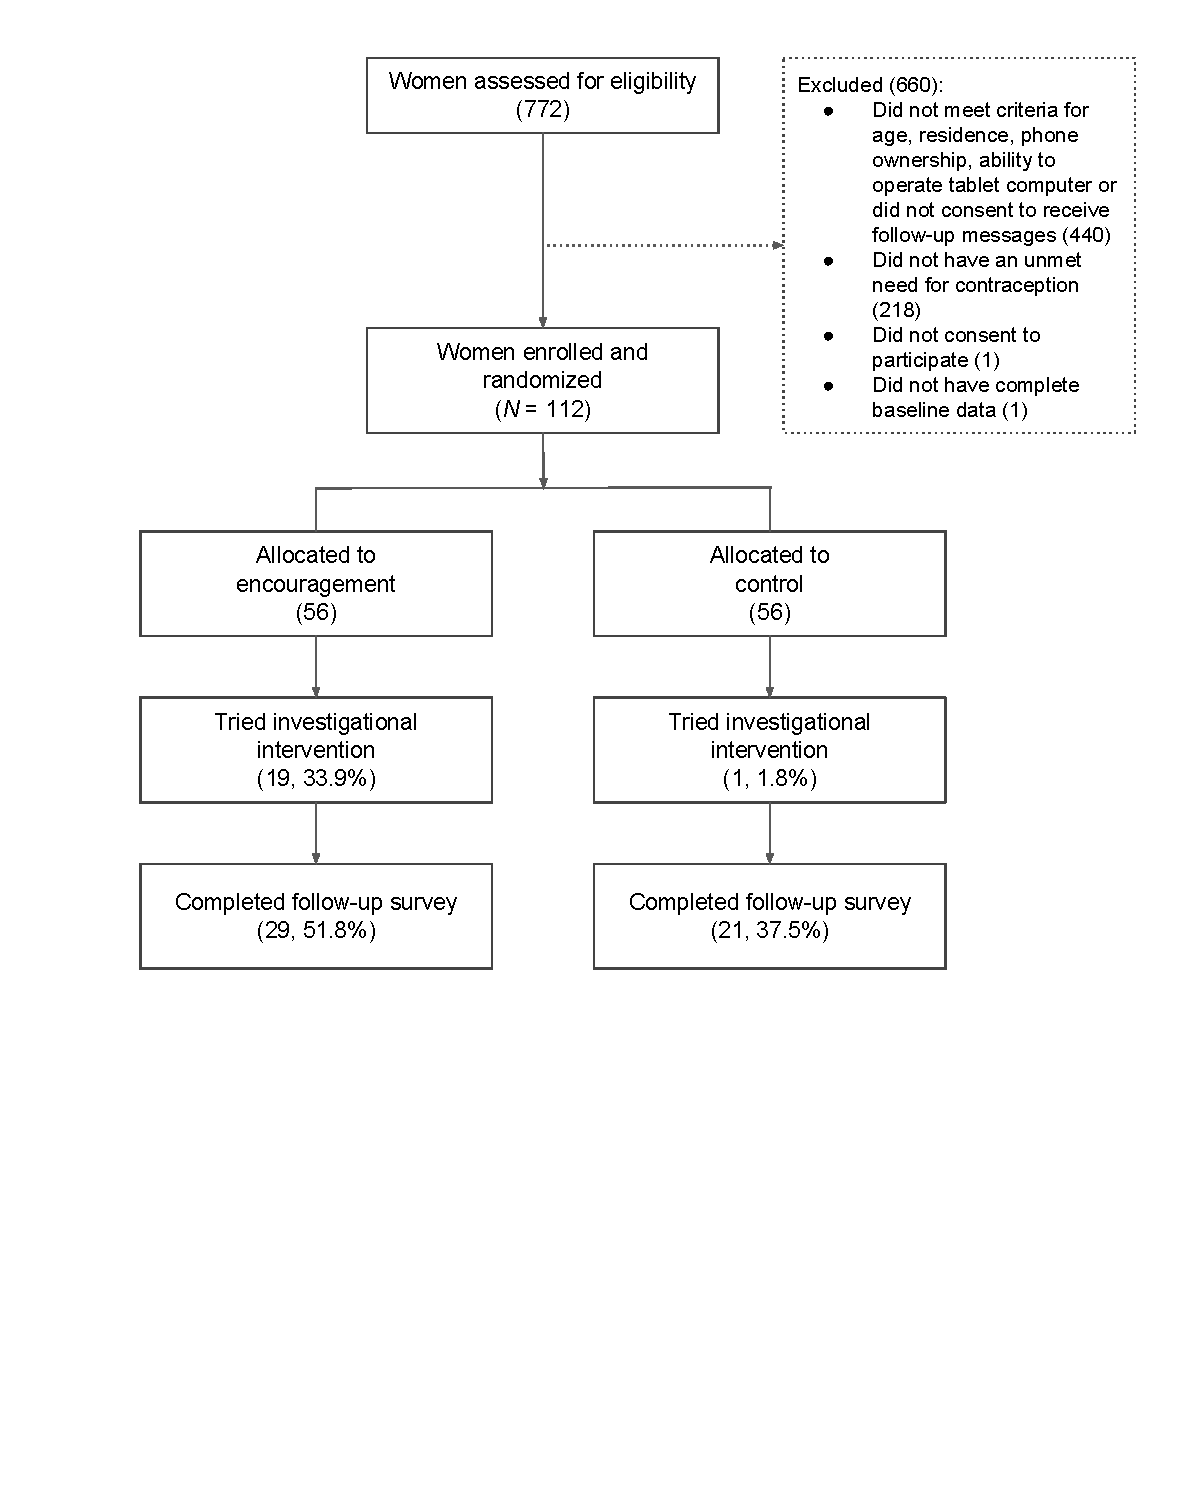
\includegraphics{../../input/figures/flow.pdf}
\caption{\label{fig:flow}Participant flow diagram.}
\end{figure}

\hypertarget{intervention}{%
\subsection{Intervention}\label{intervention}}

The investigational intervention was a digital health marketplace for
family planning called Nivi {[}13{]}. At the time of the study, any
woman (or man) in Bungoma county could send a toll-free SMS message to
the Nivi service to ask a question about reproductive health or trigger
a free callback to complete an automated family planning counseling
session via interactive voice response. This screening resulted in a set
of recommended methods that fit the client's preferences and goals,
along with referrals to local public and private providers offering one
or more of these methods. After a period of time, clients were prompted
to provide details about their experience with family planning providers
and were eligible to receive a transportation voucher (approximately USD
\$2) as a nudge toward behavior change.

\hypertarget{experimental-design-and-randomization}{%
\subsection{Experimental Design and
Randomization}\label{experimental-design-and-randomization}}

Since the service was available to anyone living in Bungoma county, it
was not possible to restrict access and estimate impact of the service
through a randomized controlled trial. In situations like this, a
randomized encouragement design can be very effective {[}14{]}. In a
randomized encouragement design, participants are randomized to receive
an invitation or special encouragement to receive an intervention. Not
everyone who is encouraged will try the intervention (and some who are
not invited will try on their own), but as long as those randomly
assigned to receive the encouragement---\enquote{the treatment
group}---try the intervention at a higher rate than those not
encouraged---the \enquote{control group}---it is possible to estimate
the impact of the intervention. This design has been used to study a
variety of interventions where two-sided non-compliance is possible
{[}15--18{]}.

In this pilot trial, we randomly allocated the sample of 112 enrolled
women to the treatment or control arm (1:1). At the end of the
recruitment period, the first author used the \texttt{blockTools}
package {[}19{]} in R {[}20{]} to block randomization on age and
baseline indicators of having attended postsecondary schooling, previous
use and discontinuation of contraception, and being married or living in
a union. One month after the end of the recruitment period, on October
2, 2017, women randomized to the encouragement arm received an
invitation via SMS to text the service and complete a free family
planning screening (plus bonus phone credit of approximately USD \$2,
not conditional on use of the service). Women randomized to the control
arm received a different set of messages thanking them for participating
in the study; the control messages did not mention the investigational
service.

\hypertarget{outcome-data-collection}{%
\subsection{Outcome Data Collection}\label{outcome-data-collection}}

We conducted a follow-up survey between February 14 and March 13, 2018,
approximately four months after we invited the treatment group to try
the service. Participants could complete the survey for free via SMS in
their preferred language or choose to receive a free callback from a
study enumerator to complete the survey over the phone. Any woman who
attempted SMS but experienced an error was flagged for enumerator
follow-up. The study enumerator was blind to each participant's
assignment until the end of the survey. We sent up to four SMS reminders
to study participants who did not reply. Women who completed the survey
received an honorarium of Ksh 200 (approximately USD \$2) to appreciate
their time and effort.

The primary outcome under investigation was self-reported use of a
modern method of contraception {[}21{]} since the baseline
survey.\footnote{The reference point for the start of the recall period
  was the national election conducted on August 8, 2017, several days
  after the end of the baseline survey.} This included women who adopted
and subsequently discontinued a method during this period. We obtained a
binary indicator of attempted service use by querying the system logs
for participant phone numbers. If a participant's phone number was
present in the system logs, we coded her as having tried the service.

\hypertarget{statistical-methods}{%
\subsection{Statistical Methods}\label{statistical-methods}}

Because encouragement designs lead to two-sided non-compliance, we
planned to use instrumental variables regression to obtain an unbiased
Local Average Treatment Effect (LATE) of the impact of service use on
contraceptive uptake. We used the \texttt{AER} {[}22{]} package in R
{[}20{]} to estimate LATE via two-stage least squares regression. In the
first stage, we regressed the indicator of service use on the
instrumental variable---a binary indicator of random assignment to the
treatment group. In the second stage, we regressed the primary outcome
of contraceptive uptake on the predicted values of service use from the
first stage regression. Both regressions included baseline controls and
the mode of follow-up survey. We used the \texttt{ivpack} {[}23{]}
package to obtain corrected Huber-White standard errors. Results of
non-linear specifications are presented in the Appendix.

One aim of the study was to test the recruitment procedures and examine
the potential for attrition. We based the target sample size for the
full trial on the assumption that a sample size of 50 would be needed in
an individually randomized trial (25 per arm) to detect a difference in
contraception uptake of 30 percentage points between the control group
(10\%) and the treatment group (40\%), given alpha of 5\%, power of
80\%, and a one-tailed test. We increased this sample size estimate by a
factor of 2.8 to account for the fact that only a subset of the
treatment group was expected to take up the intervention (70\%) and that
there would be a differential rate of service uptake in the control
group that was not encouraged (10\%). The inflation factor was
\(1/(0.7-0.1)^2\), producing an adjusted target sample size of 139
{[}24{]}.

\hypertarget{ethical-review}{%
\subsection{Ethical Review}\label{ethical-review}}

Institutional Review Boards at Duke University and Moi University
reviewed and approved this study protocol. This pilot study is
registered with ClinicalTrials.gov (NCT03224390).

\hypertarget{results}{%
\section{Results}\label{results}}

\hypertarget{participant-characteristics}{%
\subsection{Participant
Characteristics}\label{participant-characteristics}}

As shown in Figure \ref{fig:flow}, we assessed 772 women for eligibility
and enrolled 112. A total of 660 women were excluded because they did
not meet the inclusion criteria; 33.0\% of excluded women had a met need
for contraception.

Table \ref{tbl-part} summarizes characteristics of the enrolled sample.
The average age of participants was 24.7 (\emph{SD}=4.8 years). The
majority of women in the study were married or in a union, and
two-thirds reported previous pregnancies. The average woman gave birth
to 1.6 (\emph{SD}=1.6) children and desired to have a total of 3.6
(\emph{SD}=1.3) children. Therefore, most reported an unmet need for
spacing rather than limiting. As is typical of women in Bungoma county
according to the most recent DHS, the women in this study were familiar
with family planning methods. Most women indicated that they had
recently been exposed to family planning messages in the media, and the
average woman said she had heard of 9.6 (\emph{SD}=2.2) out of 12
methods assessed.

\begin{table}
\rotatebox[origin=c]{90}{
\scalebox{1}{
\centerline{\begin{threeparttable}
  \caption{Participant characteristics}
  \label{tbl-part}
  \centering
  \begin{tabular}{lrrrl}
  \toprule
  & & & \multicolumn{2}{c}{Kenya DHS 2014 Reference} \\
  \cline{4-5}
  Characteristic & Control & Treatment & Value & Group \\
  \midrule
  \expandableinput ../../output/tables/part.tex
  \bottomrule
  \end{tabular}
  \begin{tablenotes}
  \small
  \item Note. $^a$ currently married women with an unmet need for family planning. $^b$ women who started an episode of contraceptive use within the five years preceding the survey and discontinued within 12 months. $^c$ Asked about knowledge of 12 different methods. $^d$ Did not hear or see a family planning message on radio, on television or in a newspaper or magazine in the past few months.
  \end{tablenotes}
  \end{threeparttable}}}\hspace{1in}
}
\end{table}

\hypertarget{intervention-take-up}{%
\subsection{Intervention Take-Up}\label{intervention-take-up}}

The randomized encouragement design had only a modest effect on the
probability of trying the intervention. Four months after the treatment
group was encouraged via SMS to try the service, 19 women (33.9\%) in
the treatment group initiated a session. This compares to 1 women
(1.8\%) in the control group. The encouragement did produce a
differential rate of take-up of 32.1 percentage points, but the
difference was smaller than anticipated.

Table \ref{tbl-corr} shows the correlates of intervention use among the
treatment group. Age was negatively associated with use, which was
expected. No other baseline characteristics of participants were
significantly associated with use.

\begin{table}[!htbp] \centering 
  \caption{Correlates of intervention take up (among treatment group)} 
  \label{tbl-corr} 
\begin{tabular}{@{\extracolsep{5pt}}lc} 
\\[-1.8ex]\hline 
\hline \\[-1.8ex] 
 & \multicolumn{1}{c}{\textit{Dependent variable:}} \\ 
\cline{2-2} 
\\[-1.8ex] & Tried intervention \\ 
\hline \\[-1.8ex] 
 Age & $-$0.04$^{*}$ (0.02) \\ 
  Is married or in a union & $-$0.16 (0.20) \\ 
  Identifies as Christian & 0.44 (0.33) \\ 
  Identifies as member of Luhya tribe & $-$0.01 (0.18) \\ 
  Attended post-secondary schooling & 0.20 (0.17) \\ 
  Is nulligravida & 0.09 (0.24) \\ 
  Number of children born & 0.04 (0.10) \\ 
  Desired number of children & 0.06 (0.09) \\ 
  Has unmet need for spacing & $-$0.03 (0.24) \\ 
  Past use of family planning & $-$0.26 (0.17) \\ 
  Number of methods known & 0.01 (0.03) \\ 
  Not exposed to family planning messages & $-$0.19 (0.20) \\ 
  Constant & 0.71 (0.58) \\ 
 \hline \\[-1.8ex] 
Mean of dependent variable & 0.34 \\ 
Observations & 56 \\ 
R$^{2}$ & 0.28 \\ 
Adjusted R$^{2}$ & 0.08 \\ 
Residual Std. Error & 0.46 (df = 43) \\ 
F Statistic & 1.40 (df = 12; 43) \\ 
\hline 
\hline \\[-1.8ex] 
\multicolumn{2}{l} {\parbox[t]{11cm}{ \textit{Notes:} Sample limited to women randomly assigned to the treatment group. Coefficients estimated through linear probability model regression. Standard errors in parentheses.\\ $^{*}$p$<$0.1; $^{**}$p$<$0.05; $^{***}$p$<$0.01}} \\
\end{tabular} 
\end{table}

\hypertarget{study-attrition}{%
\subsection{Study Attrition}\label{study-attrition}}

As shown in Figure \ref{fig:flow}, there was a substantial amount of
attrition. We obtained follow-up data from 44.6\% of enrolled
participants. Table \ref{tbl-att} shows that attrition was higher among
the control group, but this difference was not statistically significant
at conventional levels. Attrition was significantly associated with a
few baseline characteristics, including post-secondary education,
nulligravida, and mean number of children born; found participants were
more likely to have attended post-secondary schooling, have never been
pregnant, and have fewer children. The impact analysis controls for
these baseline characteristics and the mode of survey administration.
Slightly more than half of these participants (56.0\%) completed the
follow-up survey via SMS (versus via phone call with a study
enumerator). Missing follow-up observations were imputed with baseline
values (last observation carried forward), which in this study was no
contraceptive use on study entry.

\begin{table}
\rotatebox[origin=c]{0}{
\scalebox{1}{
\centerline{\begin{threeparttable}
  \caption{Baseline participant characteristics by follow-up status}
  \label{tbl-att}
  \centering
  \begin{tabular}{lrrr}
  \toprule
  Characteristic & Not Found (\textit{n}=62) & Found (\textit{n}=50) & \textit{p}-value \\
  \midrule
  \expandableinput ../../output/tables/att.tex
  \bottomrule
  \end{tabular}
  \begin{tablenotes}
  \small
  \item Note. Two-sample t-tests of mean differences and two-proportions z-tests of differences in proportions. $^a$ Asked about knowledge of 12 different methods. $^b$ Did not hear or see a family planning message on radio, on television or in a newspaper or magazine in the past few months.\\ $^{*}$p$<$0.1; $^{**}$p$<$0.05; $^{***}$p$<$0.01
  \end{tablenotes}
  \end{threeparttable}}}\hspace{1in}
}
\end{table}

\hypertarget{effects-of-intervention-use}{%
\subsection{Effects of Intervention
Use}\label{effects-of-intervention-use}}

Table \ref{tbl-impact} presents preliminary evidence of the impact of
the investigational intervention on contraception adoption. Assignment
to the treatment group led to an increase of 12.7 percentage points in
the likelihood of contraception use. Among actual users of the
intervention, the instrumental variables estimate suggests that this
effect was 41.0 percentage points. The sign of the instrumental
variables estimate appears to be positive, but the confidence interval
is wide.

\begin{table}[!htbp] \centering 
  \caption{Impact on contraception adoption} 
  \label{tbl-impact} 
\begin{tabular}{@{\extracolsep{5pt}}lccc} 
\\[-1.8ex]\hline 
\hline \\[-1.8ex] 
\\[-1.8ex] & \textit{First stage} & \textit{ITT estimation} & \textit{IV estimation} \\ 
 & Tried intervention & Adopted contraception & Adopted contraception \\ 
\\[-1.8ex] & (1) & (2) & (3)\\ 
\hline \\[-1.8ex] 
 Assigned to treatment & 0.31$^{***}$ & 0.13$^{*}$ &  \\ 
  & (0.19, 0.44) & ($-$0.01, 0.26) &  \\ 
  & & & \\ 
 Tried intervention &  &  & 0.41$^{*}$ \\ 
  &  &  & ($-$0.03, 0.85) \\ 
  & & & \\ 
\hline \\[-1.8ex] 
Mean in control group & 0.02 & 0.16 &  \\ 
Includes controls & Yes & Yes & Yes \\ 
Observations & 112 & 112 & 112 \\ 
\hline 
\hline \\[-1.8ex] 
\multicolumn{4}{l} {\parbox[t]{17cm}{ \textit{Notes:} The first stage regression estimate (Column 1) is the coefficient on assignment to treatment from an OLS regression of intervention use on assignment. The intent-to-treat (ITT) estimate (Column 2) is the coefficient on assignment to treatment from an OLS regression of contraception adoption on assignment. The instrumental variables (IV) estimate (Column 3) is the coefficient on intervention use in a two-stage least squares regression of contraception adoption on assignment and intervention use. Controls include an indicator for mode of follow-up survey administration and several baseline characteristics, including: age, number of children born, and indicators for having attended post-secondary schooling, past use of family planning, being married or in a union, and nulligravida. Corrected Huber-White standard errors. \\ $^{*}$p$<$0.1; $^{**}$p$<$0.05; $^{***}$p$<$0.01}} \\
\end{tabular} 
\end{table}

Two additional specifications are presented in the Appendix. Table
\ref{tbl-impact-noimpute} displays the OLS estimates produced without
the use of last observation carried forward imputation. In these models,
the estimates and confidence intervals are slightly larger than what is
presented in Table \ref{tbl-impact}. Table \ref{tbl-impact-probit}
presents the results of probit regressions; the results of these
non-linear specifications are consistent with the linear results
presented in Table \ref{tbl-impact}.

\hypertarget{discussion}{%
\section{Discussion}\label{discussion}}

This pilot study demonstrates that the proposed recruitment,
encouragement, and data collection procedures are feasible, but some
modifications are necessary prior to conducting a full trial.
Additionally, analysis of the pilot data suggests that the
investigational intervention has a positive effect on contraceptive
take-up among women with an unmet need in Kenya, but a full trial is
required to more precisely estimate the magnitude of this effect.

During a recruitment period that lasted four weeks, we screened 772
women for eligibility, but only enrolled 14.5\% in the study. At this
rate, it would have taken another week to reach our original target
sample size. While this approach was feasible in terms of time and
resources, it was inefficient in two ways. First, two-thirds of women
who were ineligible to enroll did not meet basic eligibility criteria
such as age, residence, and phone ownership. Screening out these women
was not time intensive, but we could have eliminated some work and
inconvenience to interested women by more clearly stating the criteria
on the market stall signage. Second, 1 out of every 3 ineligible women
were ineligible because they did not have an unmet need for family
planning. To some extent this was unavoidable because we did not recruit
directly for women with an unmet need, but rather embedded checks for
eligibility in a short screening available to all women in the eligible
age range. However, in a future trial it may be advantageous to recruit
from other sub-populations in addition to open-air markets to increase
the probability that the pool of potential participants will have an
unmet need. For instance, recruiting from post-secondary institutions
would enable us to reach younger, unmarried women who may be sexually
active but not using contraception. Postnatal clinics are another
potential venue for recruitment as there is a high unmet need among new
mothers in this region.

We used a randomized encouragement design to account for expected
two-sided non-compliance with treatment assignment. Women assigned to
the treatment group received an invitation via text message to try the
intervention, and 33.9\% of those invited accepted the invitation, a
conversion rate that appears to be consistent with SMS marketing
conversion rates observed in industry {[}25{]}. By comparison, 1.8\% of
control participants tried the intervention. The encouragement led to a
differential rate of intervention take-up of 32.1 percentage points,
thereby making causal identification possible using assignment to
treatment as an instrument.

The intervention take-up rate is important because incomplete take-up
requires an inflation of sample size estimates that are based on fixed
parameters for power, alpha, and the desired minimal detectable effect
size for traditional randomized controlled trials. Another important
consideration for the optimal sample size is attrition. In this study,
44.6\% of enrolled participants completed the follow-up survey via SMS
or phone call with a study enumerator. We did not collect detailed
tracking information from participants during the recruitment process,
so we could only invite participants to complete the survey via SMS. In
a future trial, it will be important to have the option to conduct
in-person follow-up to reduce study attrition. Other studies that relied
solely on SMS-invite as we did have encountered similar challenges
{[}8{]}.

A third key consideration for sample size calculations is the minimal
detectable effect size. In this study, the instrumental variables
estimate of the treatment effect was an increase in the likelihood of
contraception take-up of 41.0 percentage points among treatment group
members who tried the intervention. This is an approximate standardized
effect size of 1.1. This is only a point estimate, however. The 95\%
confidence interval is wide. While the results suggest that the
intervention effect is positive, the point estimate is not measured
precisely. The effect observed in this study would be large relative to
other SMS interventions for health behavior change {[}8,26{]}, so it
will be important to use a more conservative estimate to determine the
optimal sample size for the full trial.

\hypertarget{limitations}{%
\subsection{Limitations}\label{limitations}}

The main limitation of this study is attrition. While attrition was not
significantly associated with treatment assignment, found and unfound
participants differed on a few baseline characteristics. The preliminary
impact analysis controls for these differences, but selection bias is a
concern. Our reliance on self-reported data, while standard for a trial
like this, also has the potential for bias.

As this study was conducted in only one, largely rural county in Kenya,
the results may not generalize to urban or international markets.
Additionally, the study was conducted at a unique and challenging time.
A few days after the end of the recruitment period, Kenyans voted in a
national election that was ultimately nullified by the Supreme Court. A
second election took place on October 26, 2017, roughly two weeks after
the treatment group was encouraged to try the intervention. Then in
early November, a 5-month national nurse's strike came to an end, and
nurses around the country---including the bulk of the country's family
planning service providers---returned to work. In short, the pilot study
was conducted during a period of uncertainty, likely distrust of SMS
marketing amid heavy political advertising, and a significant decrease
in the availability of family planning providers.

\hypertarget{conclusions}{%
\subsection{Conclusions}\label{conclusions}}

This randomized encouragement design and study protocol is feasible but
requires modifications to the recruitment, encouragement, and follow-up
data collection procedures. The investigational intervention appears to
have a positive impact on contraceptive take-up among women with an
unmet need despite a number of contextual challenges running concurrent
to the trial.

\newpage

\hypertarget{acknowledgements}{%
\section{Acknowledgements}\label{acknowledgements}}

This research was supported by a pilot grant from the Duke Global Health
Institute. For their assistance with data collection, the authors would
like to thank Anna-Karin Hess, Lulla Kiwinda, Maximilla Chivini, Nancy
Wairmu, Mercy Murungi, and Purity Nyangweso. The authors also appreciate
feedback on study design from Dr.~Ben Bellows, Siddhartha Goyal, and the
Nivi team.

\hypertarget{conflicts-of-interest}{%
\section{Conflicts of Interest}\label{conflicts-of-interest}}

Eric Green is a Co-Founder of Nivi, Inc., holds an equity stake in the
company, is a member of the company's Board of Directors, and serves as
the company's Chief Scientist. Green is a faculty member in the Duke
Global Health Institute. Duke University also holds an equity stake in
the company. Green's potential conflicts of interest are managed by Duke
University's Research Integrity Office (MP\#0600050-2017-001-A).

\hypertarget{abbreviations}{%
\section{Abbreviations}\label{abbreviations}}

ITT: Intent-to-treat

IV: Instrumental variables

DHS: Demographic and Health Survey

LATE: Local Average Treatment Effect

SMS: short message service

\newpage

\hypertarget{references}{%
\section{References}\label{references}}

\setlength{\parindent}{-0.5in}\setlength{\leftskip}{0.5in}

\hypertarget{refs}{}
\leavevmode\hypertarget{ref-bongaarts:2012}{}%
1. Bongaarts J, Cleland J, Townsend JW, Bertrand JT, Gupta M. Family
Planning Programs For the 21st Century. New York: Population Council;
2012.

\leavevmode\hypertarget{ref-fp2020:2017}{}%
2. FP2020. FP2020: The Way Ahead {[}Internet{]}. FP2020; 2017. Report
No.: 2016-2017. Available from:
\url{http://progress.familyplanning2020.org/en}

\leavevmode\hypertarget{ref-kenyanationalbureauofstatistics:2015}{}%
3. Statistics KNB of, Health KM of, Council NAC, Institute KMR,
Population NC for, Development, The DHS Program II. Kenya Demographic
and Health Survey 2014. Nairobi, Kenya: KNBS; 2015.

\leavevmode\hypertarget{ref-kenyanationalbureauofstatistics:2014}{}%
4. Statistics KNB of, Health KM of, Council NAC, Institute KMR,
Population NC for, Development. Kenya Demographic and Health Survey 2014
Key Indicators. Nairobi, Kenya: Kenya National Bureau of Statistics;
2014.

\leavevmode\hypertarget{ref-mwaikambo:2011}{}%
5. Mwaikambo L, Speizer IS, Schurmann A, Morgan G, Fikree F. What works
in family planning interventions: A systematic review of the evidence.
Stud Fam Plann {[}Internet{]} 2011 Jun {[}cited 2018 Mar
14{]};42(2):67--82. Available from:
\url{https://www.ncbi.nlm.nih.gov/pmc/articles/PMC3761067/}

\leavevmode\hypertarget{ref-labrique:2013}{}%
6. Labrique AB, Vasudevan L, Kochi E, Fabricant R, Mehl G. mHealth
innovations as health system strengthening tools: 12 common applications
and a visual framework. Global Health: Science and Practice
{[}Internet{]} 2013 Aug 1 {[}cited 2018 Mar 14{]};1(2):160--171. {[}doi:
\href{https://doi.org/10.9745/GHSP-D-13-00031}{10.9745/GHSP-D-13-00031}{]}

\leavevmode\hypertarget{ref-gurman:2012}{}%
7. Gurman TA, Rubin SE, Roess AA. Effectiveness of mHealth Behavior
Change Communication Interventions in Developing Countries: A Systematic
Review of the Literature. Journal of Health Communication {[}Internet{]}
2012 May 2 {[}cited 2018 Mar 14{]};17(sup1):82--104. {[}doi:
\href{https://doi.org/10.1080/10810730.2011.649160}{10.1080/10810730.2011.649160}{]}

\leavevmode\hypertarget{ref-johnson:2017}{}%
8. Johnson D, Juras R, Riley P, Chatterji M, Sloane P, Choi SK, Johns B.
A randomized controlled trial of the impact of a family planning mHealth
service on knowledge and use of contraception. Contraception
{[}Internet{]} 2017 Jan 1 {[}cited 2018 Mar 14{]};95(1):90--97. {[}doi:
\href{https://doi.org/10.1016/j.contraception.2016.07.009}{10.1016/j.contraception.2016.07.009}{]}

\leavevmode\hypertarget{ref-wittes:1990}{}%
9. Wittes J, Brittain E. The role of internal pilot studies in
increasing the efficiency of clinical trials. Statistics in Medicine
1990;9(1-2):65--72.

\leavevmode\hypertarget{ref-lancaster:2004}{}%
10. Lancaster GA, Dodd S, Williamson PR. Design and analysis of pilot
studies: Recommendations for good practice. Journal of evaluation in
clinical practice 2004;10(2):307--312.

\leavevmode\hypertarget{ref-bradley:2012}{}%
11. Bradley SE, Croft TN, Fishel JD, Westoff CF. Revising unmet need for
family planning. Calverton, Maryland: ICF International and MEASURE DHS;
2012. Report No.: 25.

\leavevmode\hypertarget{ref-bradley:2014}{}%
12. Bradley SE, Casterline JB. Understanding Unmet Need: History,
Theory, and Measurement. Stud Fam Plann {[}Internet{]} 2014 Jun {[}cited
2018 Mar 2{]};45(2):123--150. {[}doi:
\href{https://doi.org/10.1111/j.1728-4465.2014.00381.x}{10.1111/j.1728-4465.2014.00381.x}{]}

\leavevmode\hypertarget{ref-nivi:2018}{}%
13. Nivi. Nivi {[}Internet{]}. 2018. Available from:
\url{http://nivi.io/}

\leavevmode\hypertarget{ref-west:2008}{}%
14. West SG, Duan N, Pequegnat W, Gaist P, Des Jarlais DC, Holtgrave D,
Szapocznik J, Fishbein M, Rapkin B, Clatts M, Mullen PD. Alternatives to
the Randomized Controlled Trial. Am J Public Health 2008
Aug;98(8):1359--1366. {[}doi:
\href{https://doi.org/10.2105/AJPH.2007.124446}{10.2105/AJPH.2007.124446}{]}

\leavevmode\hypertarget{ref-duflo:2003}{}%
15. Duflo E, Saez E. The role of information and social interactions in
retirement plan decisions: Evidence from a randomized experiment. The
Quarterly Journal of Economics 2003;118(3):815--842.

\leavevmode\hypertarget{ref-devoto:2012}{}%
16. Devoto F, Duflo E, Dupas P, Parienté W, Pons V. Happiness on tap:
Piped water adoption in urban Morocco. American Economic Journal:
Economic Policy 2012;4(4):68--99.

\leavevmode\hypertarget{ref-holland:1988}{}%
17. Holland PW. Causal inference, path analysis and recursive structural
equations models. ETS Research Report Series 1988;1988(1).

\leavevmode\hypertarget{ref-hirano:2000}{}%
18. Hirano K, Imbens GW, Rubin DB, Zhou X-H. Assessing the effect of an
influenza vaccine in an encouragement design. Biostatistics
2000;1(1):69--88.

\leavevmode\hypertarget{ref-blocktools}{}%
19. Moore RT. BlockTools: Blocking, assignment, and diagnosing
interference in randomized experiments. 2016.

\leavevmode\hypertarget{ref-rcore}{}%
20. R Core Team. R: A language and environment for statistical computing
{[}Internet{]}. Vienna, Austria: R Foundation for Statistical Computing;
2017. Available from: \url{https://www.R-project.org/}

\leavevmode\hypertarget{ref-who:2018}{}%
21. WHO. Family planning/Contraception {[}Internet{]}. World Health
Organization 2018. Available from:
\url{http://www.who.int/mediacentre/factsheets/fs351/en/}

\leavevmode\hypertarget{ref-aer}{}%
22. Kleiber C, Zeileis A. Applied econometrics with R {[}Internet{]}.
New York: Springer-Verlag; 2008. Available from:
\url{https://CRAN.R-project.org/package=AER}

\leavevmode\hypertarget{ref-ivpack}{}%
23. Jiang Y, Small D. Ivpack: Instrumental variable estimation.
{[}Internet{]}. 2014. Available from:
\url{https://CRAN.R-project.org/package=ivpack}

\leavevmode\hypertarget{ref-duflo:2007a}{}%
24. Duflo E, Glennerster R, Kremer M. Using randomization in development
economics research: A toolkit. Handbook of development economics
2007;4:3895--3962.

\leavevmode\hypertarget{ref-tatango:2015}{}%
25. Tatango. The Average SMS Marketing Click-Through Rate is 36\%
\textbar{} Tatango {[}Internet{]}. Tatango - SMS Marketing Software 2015
{[}cited 2018 Mar 14{]}. Available from:
\url{https://www.tatango.com/blog/the-average-sms-marketing-click-through-rate-is-36/}

\leavevmode\hypertarget{ref-armanasco:2017}{}%
26. Armanasco AA, Miller YD, Fjeldsoe BS, Marshall AL. Preventive health
behavior change text message interventions: A meta-analysis. American
Journal of Preventive Medicine 2017;52(3):391--402.





  \clearpage
  \makeatletter
  \efloat@restorefloats
  \makeatother
  
  
\begin{appendix}
\section{}
\newpage

\begin{table} \centering 
\caption{Impact on contraception adoption, sample limited to found at follow-up} 
\label{tbl-impact-noimpute} 
\begin{tabular}{@{\extracolsep{5pt}}lccc} 
\\[-1.8ex]\hline 
\hline \\[-1.8ex] 
\\[-1.8ex] & \textit{First stage} & \textit{ITT estimation} & \textit{IV estimation} \\ 
& Tried intervention & Adopted contraception & Adopted contraception \\ 
\\[-1.8ex] & (1) & (2) & (3)\\ 
\hline \\[-1.8ex] 
Assigned to treatment & 0.31$^{***}$ & 0.20 &  \\ 
& (0.19, 0.44) & ($-$0.07, 0.47) &  \\ 
& & & \\ 
Tried intervention &  &  & 0.44 \\ 
&  &  & ($-$0.15, 1.03) \\ 
& & & \\ 
\hline \\[-1.8ex] 
Mean in control group & 0.02 & 0.43 &  \\ 
Includes controls & Yes & Yes & Yes \\ 
Observations & 112 & 50 & 50 \\ 
\hline 
\hline \\[-1.8ex] 
\multicolumn{4}{l} {\parbox[t]{17cm}{ \textit{Notes:} The first stage regression estimate (Column 1) is the coefficient on assignment to treatment from an OLS regression of intervention use on assignment. The intent-to-treat (ITT) estimate (Column 2) is the coefficient on assignment to treatment from an OLS regression of contraception adoption on assignment. The instrumental variables (IV) estimate (Column 3) is the coefficient on intervention use in a two-stage least squares regression of contraception adoption on assignment and intervention use. Controls include an indicator for mode of follow-up survey administration and several baseline characteristics, including: age, number of children born, and indicators for having attended post-secondary schooling, past use of family planning, being married or in a union, and nulligravida. Corrected Huber-White standard errors. \\ $^{*}$p$<$0.1; $^{**}$p$<$0.05; $^{***}$p$<$0.01}} \\
\end{tabular} 
\end{table}

\begin{table} \centering 
\caption{Impact on contraception adoption, probit regression} 
\label{tbl-impact-probit} 
\begin{tabular}{@{\extracolsep{5pt}}lccc} 
\\[-1.8ex]\hline 
\hline \\[-1.8ex] 
\\[-1.8ex] & \textit{First stage} & \textit{ITT estimation} & \textit{IV estimation} \\ 
& Tried intervention & Adopted contraception & Adopted contraception \\ 
\\[-1.8ex] & (1) & (2) & (3)\\ 
\hline \\[-1.8ex] 
Assigned to treatment & 1.71$^{***}$ & 0.68$^{**}$ &  \\ 
& (0.54, 2.89) & (0.03, 1.34) &  \\ 
& & & \\ 
Tried intervention &  &  & 2.21* \\ 
&  &  & (-0.08, 4.5) \\ 
& & & \\ 
\hline \\[-1.8ex] 
Mean in control group & 0.02 & 0.43 &  \\ 
Includes controls & Yes & Yes & Yes \\ 
Observations & 112 & 112 & 112 \\ 
\hline 
\hline \\[-1.8ex] 
\multicolumn{4}{l} {\parbox[t]{17cm}{ \textit{Notes:} The first stage regression estimate (Column 1) is the coefficient on assignment to treatment from a probit regression of intervention use on assignment. The intent-to-treat (ITT) estimate (Column 2) is the coefficient on assignment to treatment from a probit regression of contraception adoption on assignment. The instrumental variables (IV) estimate (Column 3) is the coefficient on intervention use in a probit regression of contraception adoption on assignment and intervention use (run in Stata MP 12, Newey's two-step estimator). Controls include an indicator for mode of follow-up survey administration and several baseline characteristics, including: age, number of children born, and indicators for having attended post-secondary schooling, past use of family planning, being married or in a union, and nulligravida. \\ $^{*}$p$<$0.1; $^{**}$p$<$0.05; $^{***}$p$<$0.01}} \\
\end{tabular} 
\end{table}

\newpage

\section{}

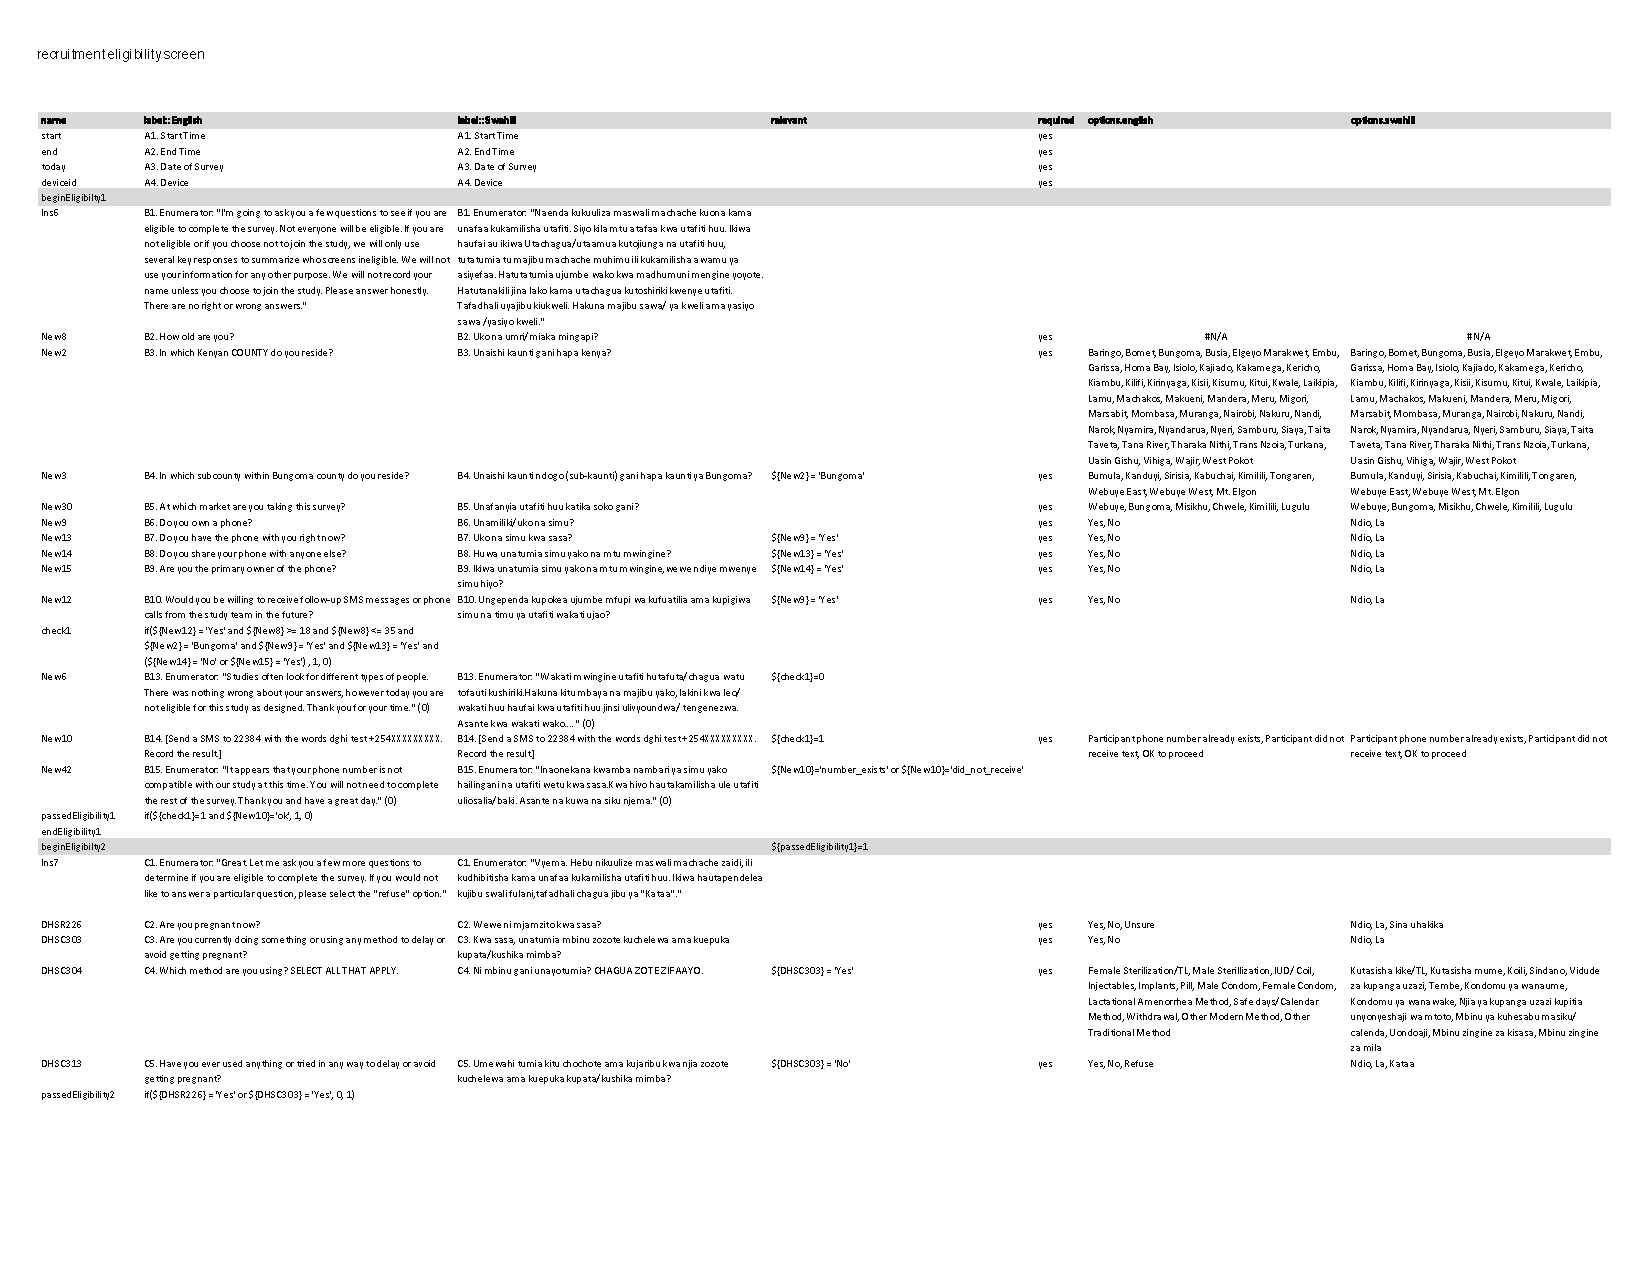
\includepdf[pages={-}, angle=90]{../../resources/survey_instruments.pdf}
\end{appendix}

\end{document}
